\subsection{Zeiterfassung}
Für die Diplomarbeit werden 180 Arbeitsstuden pro Teammitglied vorgeschrieben. Um den Arbeitsaufwand jedes Teammitglieds genau festzustellen wurde das Programm Clockify verwendet. Clockify ist ein kostenfreies Tool zur Zeiterfassung. Es gibt sowohl eine Desktop Applikation als auch eine Webanwendung. Clockify vereinfacht es die Arbeitszeit zu erfassen und zu dokumentieren. Die Zeiterfassung erfolgt über die Desktop Applikation. Die Webanwendung dient zur Auswertung der Daten. Die Daten können in verschiedenen Formaten exportiert werden. Für die Auswertung der Daten wurde Excel verwendet.


\paragraph{Arbeitsaufwand der Teammitglieder}
Die folgende Abbildung und Tabelle zeigt den Arbeitsaufwand der einzelnen Teammitglieder.

\begin{table}[!h]
  \centering
  \begin{tabular}{lr}
    \toprule
    \textbf{Teammitglied} & \textbf{Arbeitsaufwand} \\
    \midrule
    Joshua Lung           & 203 Stunden             \\
    Paul Hartmann         & 184 Stunden             \\
    Lukas Madlener        & 10 Stunden              \\
    \midrule
    Summe                 & 397 Stunden             \\
    \bottomrule
  \end{tabular}
  \caption{Arbeitsaufwand der Teammitglieder}
  \label{tab:zeiterfassung_teammitglieder}
\end{table}

\begin{figure}[!ht]
  \centering
  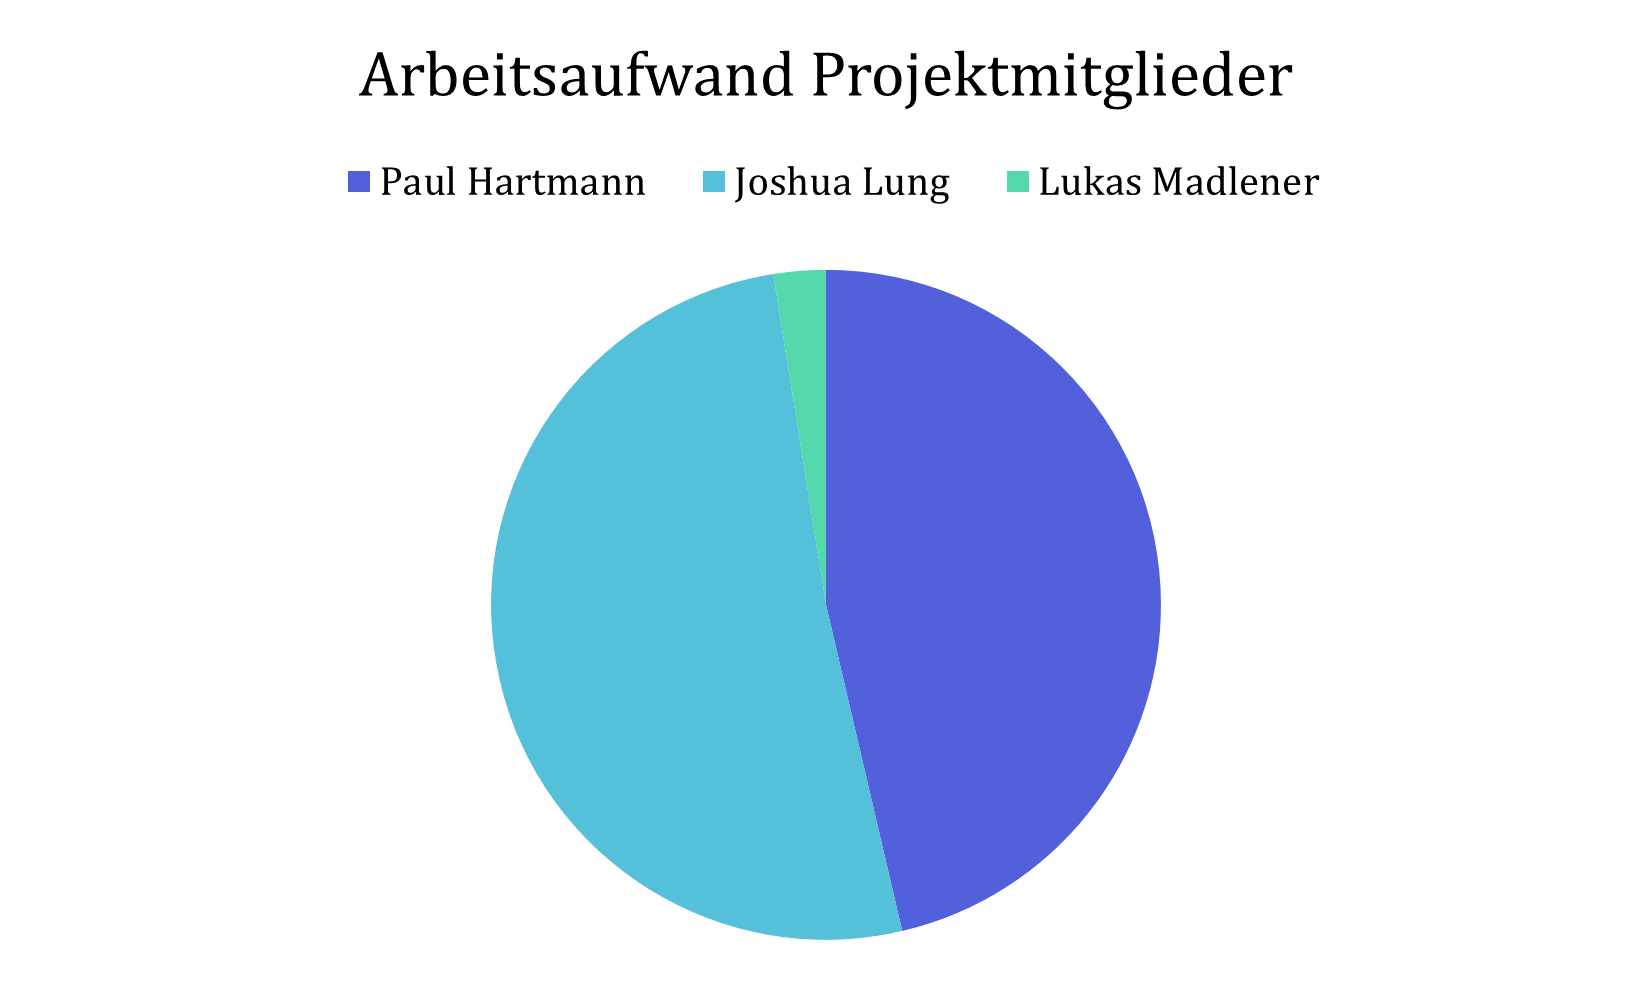
\includegraphics[width=0.8\textwidth]{images/zeiterfassung_teammitglieder.png}
  \caption{Zeitaufwand der Teammitglieder}
  \label{fig:zeiterfassung_teammitglieder}
\end{figure}


\paragraph{Arbeitsaufwand der einzelnen Projekte}
Die folgende Abbildung und Tabelle zeigt den Arbeitsaufwand der einzelnen Projekte.

\begin{table}[!h]
  \centering
  \begin{tabular}{lr}
    \toprule
    \textbf{Projekt}        & \textbf{Arbeitsaufwand} \\
    \midrule
    Schriftliche Arbeit     & 108 Stunden             \\
    Turm Controller         & 93 Stunden              \\
    Mobile App              & 83 Stunden              \\
    Sonstiges               & 43 Stunden              \\
    Recherche               & 30 Stunden              \\
    Konstruktion            & 18 Stunden              \\
    Turm Physical Prototype & 16 Stunden              \\
    Backend (Firebase)      & 3 Stunden               \\
    Admin Panel             & 3 Stunden               \\
    \midrule
    Summe                   & 397 Stunden             \\
    \bottomrule
  \end{tabular}
  \caption{Arbeitsaufwand der einzelnen Projekte}
  \label{tab:zeiterfassung_projekte}
\end{table}

\begin{figure}[!ht]
  \centering
  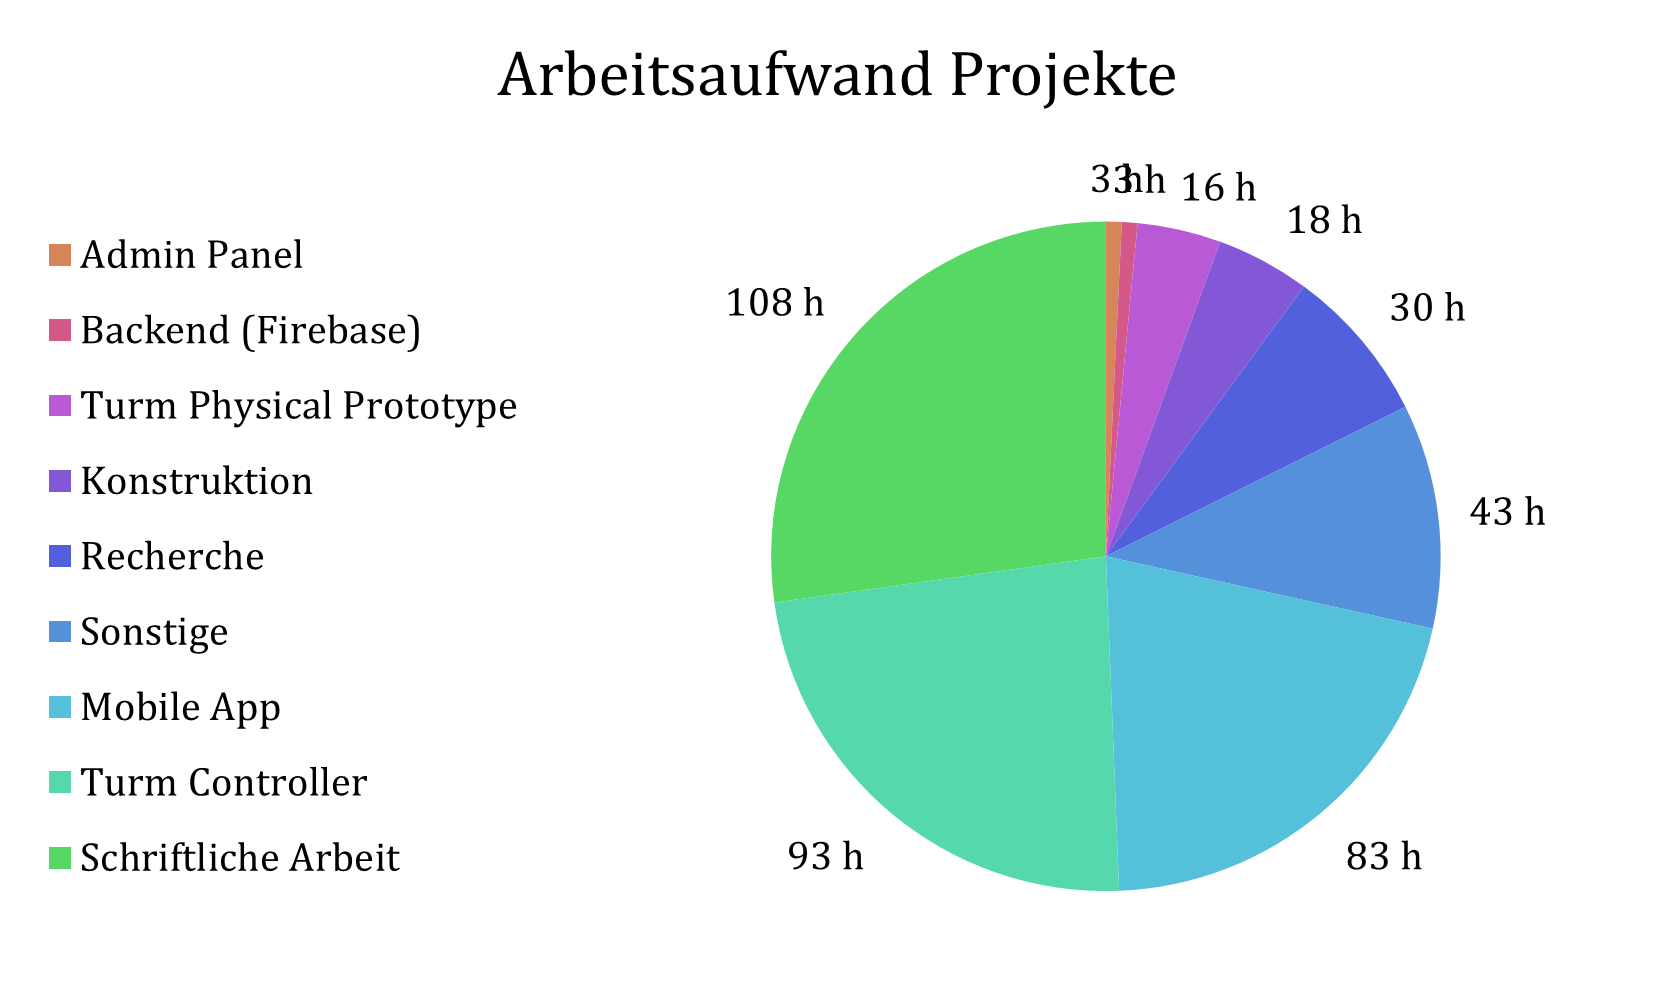
\includegraphics[width=0.8\textwidth]{images/zeiterfassung_projekte.png}
  \caption{Zeitaufwand der einzelnen Projekte}
  \label{fig:zeiterfassung_projekte}
\end{figure}


\paragraph{Arbeitsaufwand Paul Hartmann}

\begin{table}[!h]
  \centering
  \begin{tabular}{lr}
    \toprule
    \textbf{Projekt}    & \textbf{Arbeitsaufwand} \\
    \midrule
    Mobile App          & 77 Stunden              \\
    Schriftliche Arbeit & 56 Stunden              \\
    Sonstiges           & 25 Stunden              \\
    Recherche           & 13 Stunden              \\
    Konstruktion        & 7 Stunden               \\
    Admin Panel         & 3 Stunden               \\
    Backend (Firebase)  & 3 Stunden               \\
    \midrule
    Summe               & 184 Stunden             \\
    \bottomrule
  \end{tabular}
  \caption{Arbeitsaufwand Paul Hartmann}
  \label{tab:zeiterfassung_paul_hartmann}
\end{table}


\paragraph{Arbeitsaufwand Joshua Lung}

\begin{table}[!h]
  \centering
  \begin{tabular}{lr}
    \toprule
    \textbf{Projekt}        & \textbf{Arbeitsaufwand} \\
    \midrule
    Tower Controller        & 93 Stunden              \\
    Schrifliche Arbeit      & 51 Stunden              \\
    Sonstige                & 16 Stunden              \\
    Turm Physical Prototype & 16 Stunden              \\
    Recherche               & 13 Stunden              \\
    Konstruktion            & 7 Stunden               \\
    Mobile App              & 6 Stunden               \\
    \midrule
    Summe                   & 203 Stunden             \\
    \bottomrule
  \end{tabular}
  \caption{Arbeitsaufwand Joshua Lung}
  \label{tab:zeiterfassung_joshua_lung}
\end{table}


\paragraph{Arbeitsaufwand Lukas Madlener}

\begin{table}[!h]
  \centering
  \begin{tabular}{lr}
    \toprule
    \textbf{Projekt}   & \textbf{Arbeitsaufwand} \\
    \midrule
    Recherche          & 4 Stunden               \\
    Konstruktion       & 4 Stunden               \\
    Sonstiges          & 1 Stunde                \\
    Schrifliche Arbeit & 1 Stunde                \\
    \midrule
    Summe              & 10 Stunden              \\
    \bottomrule
  \end{tabular}
  \caption{Arbeitsaufwand Lukas Madlener}
  \label{tab:zeiterfassung_lukas_madlener}
\end{table}